%!TEX encoding = UTF-8 Unicode
%!TEX root = ../piccolo.tex

\cleardoublepage

\chapter{Installation et utilisation}

%--- Pour supprimer tout en-tête et pied de page sur la 1re page d'un chapitre
\thispagestyle{empty}


\section{Installation}

La page \url{http://piccolo.rts-software.org/download/index.php} contient les liens vers la distribution de Piccolo. 

Piccolo est distribué sous la forme d'un \emph{utilitaire en ligne de commande}, sauf pour Mac OS X où une application comprenant un éditeur avec coloration lexicale est proposée (voir section suivante).





\section{Application Cocoa}

Sur Mac OS X, l'application Cocoa permet d'éditer et de compiler dans le même environnement. Cette application est compatible avec \emph{Snow Leopard} (Mac OS 10.6) et les systèmes ultérieurs. Ses \emph{préférences} permettent de paramétrer :
\begin{itemize}
\item les options de compilation (\refFigure{}{cocoaOptionsCompilation}) ;
\item d'installer ou de désinstaller les outils en ligne de commande (\refFigure{}{cocoaInstallationOutilsLigneCommande}) ;
\end{itemize}


\begin{figure}[t]
  \centering
  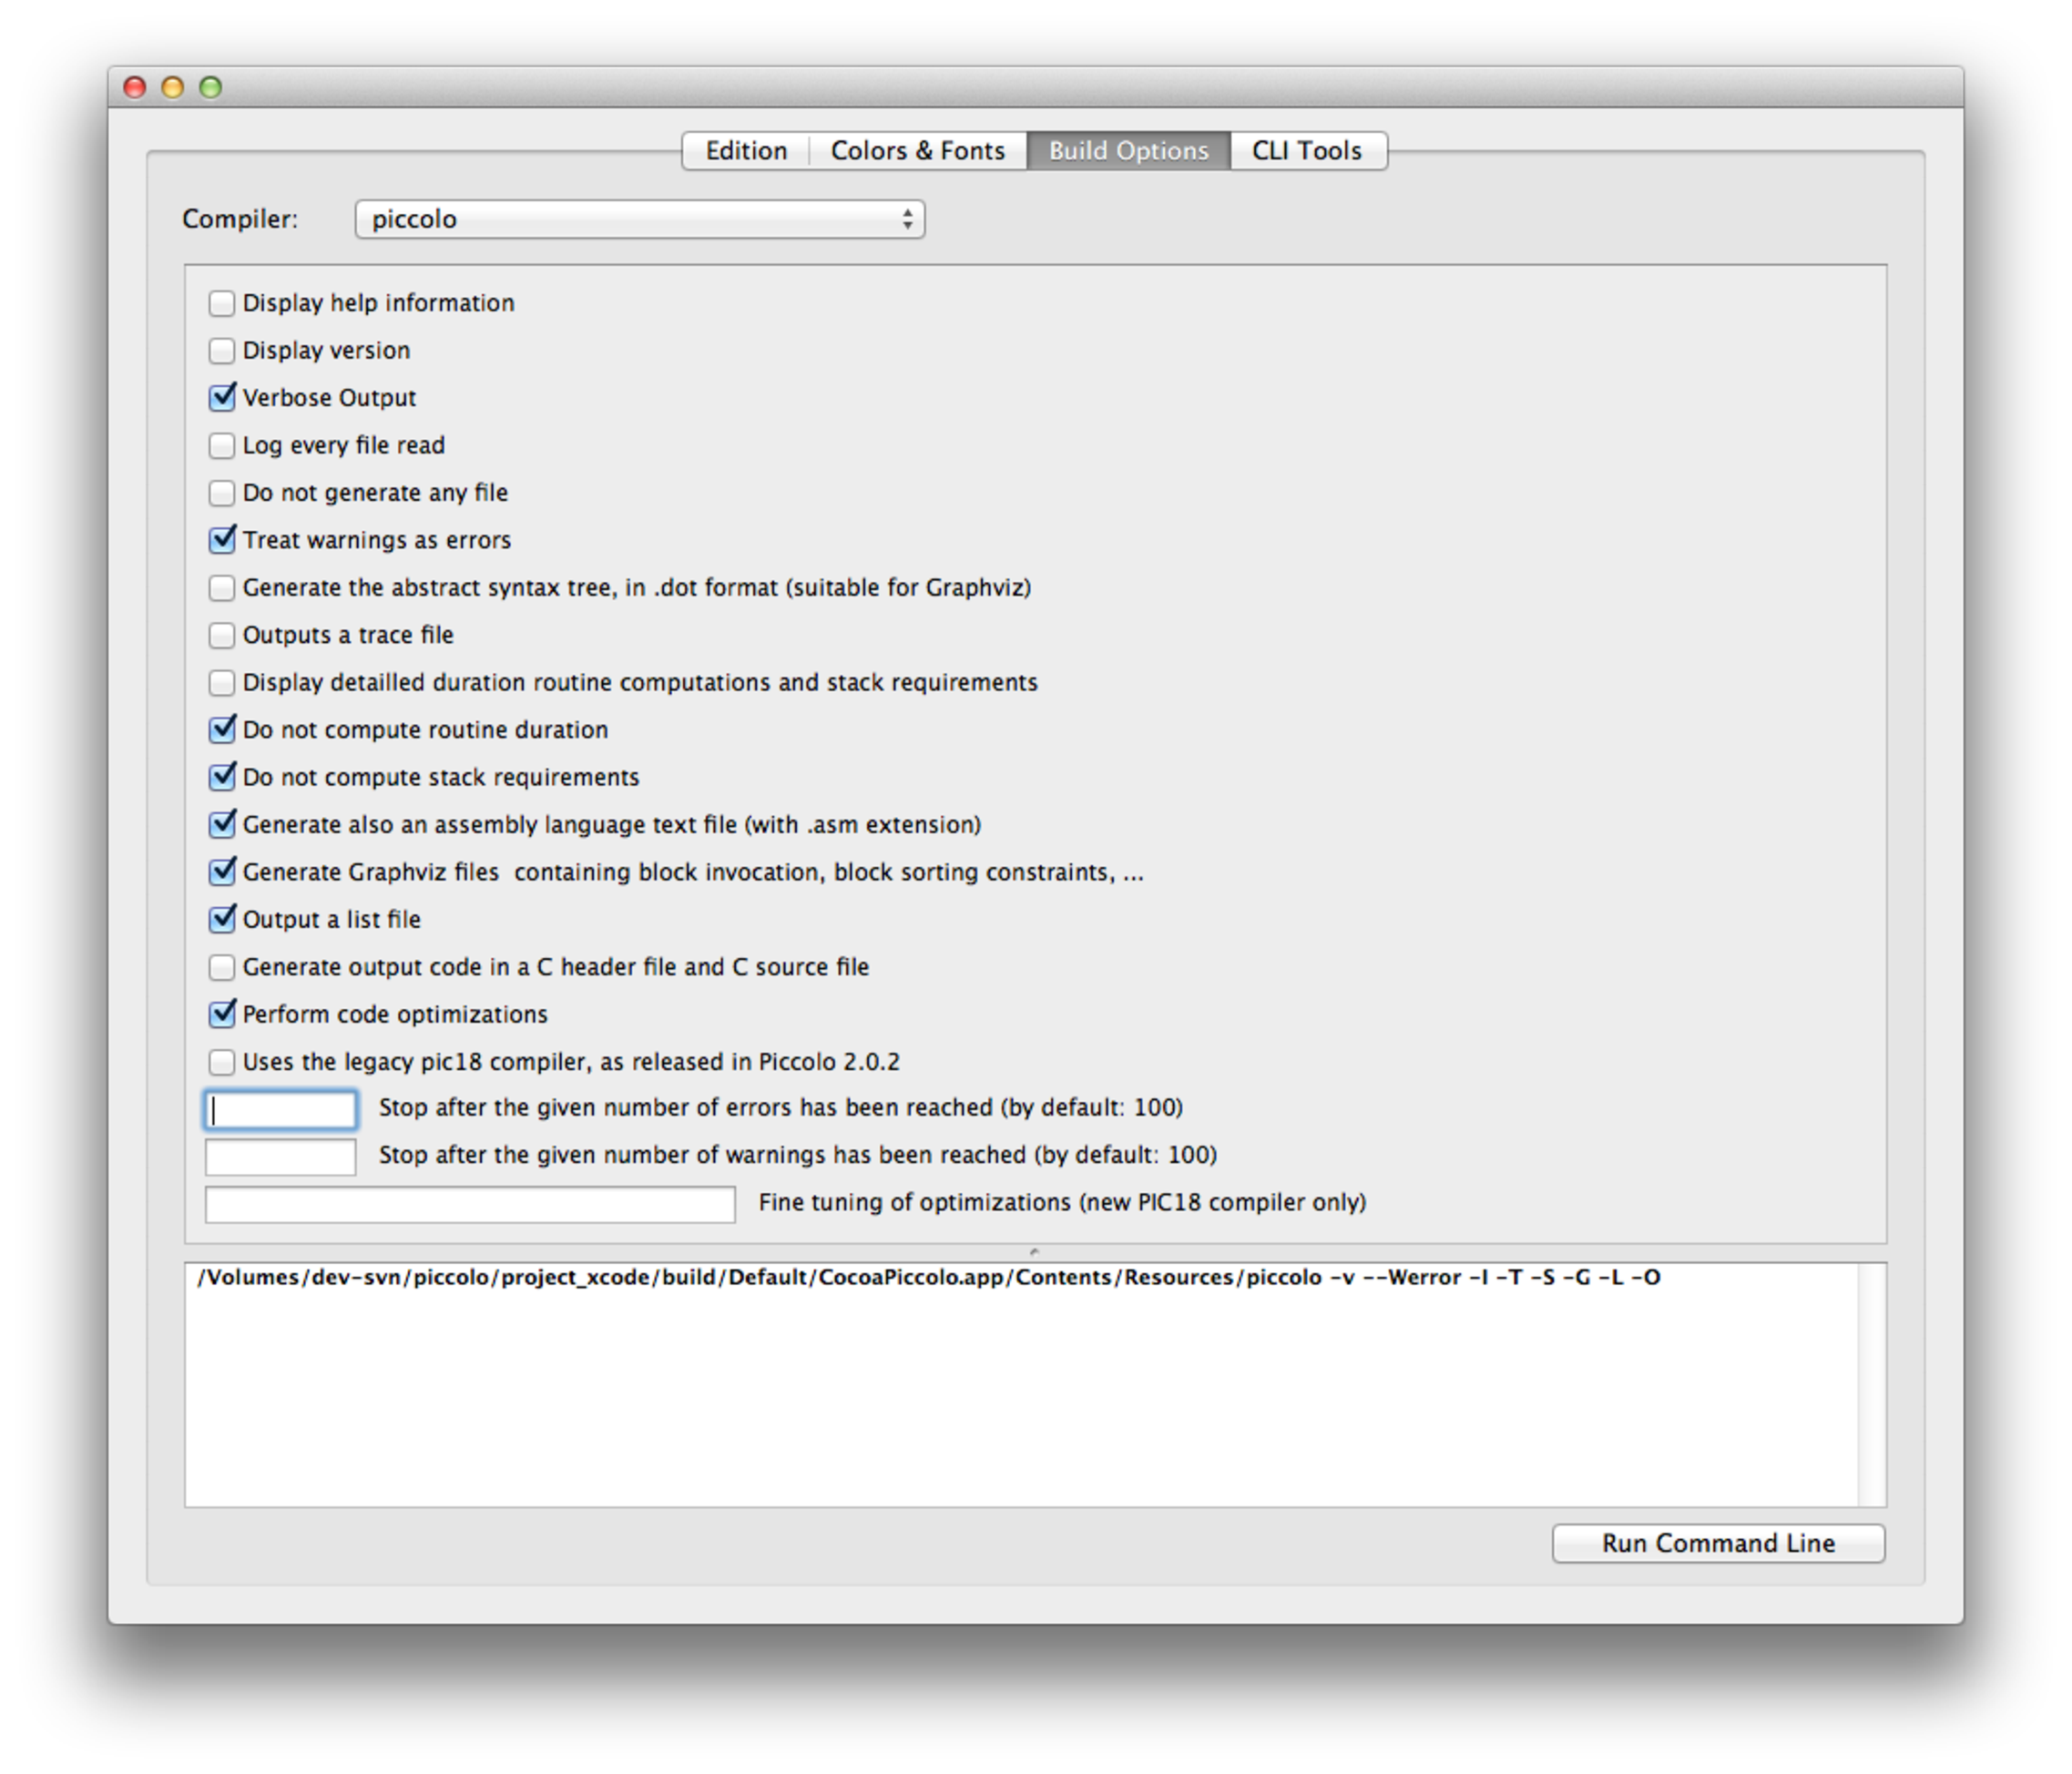
\includegraphics[width=1\textwidth]{images/build-options.pdf}
  \caption{Application Cocoa, options de compilation}
  \labelFigure{cocoaOptionsCompilation}
  \ligne
\end{figure}



\begin{figure}[t]
  \centering
  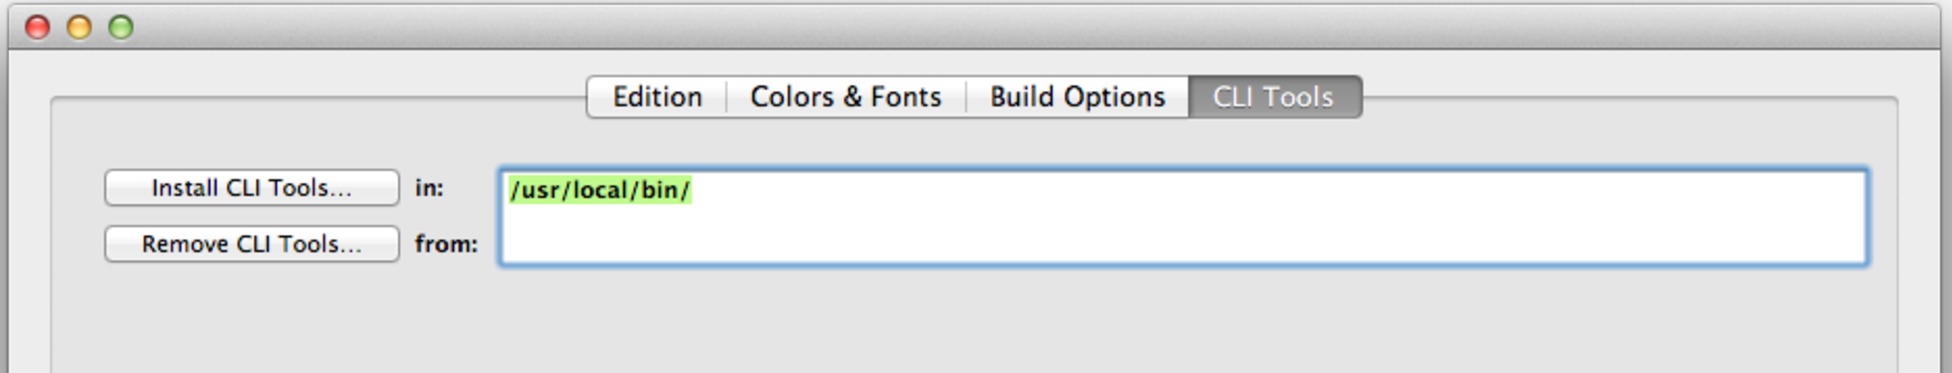
\includegraphics[width=1\textwidth]{images/installation-cli-tools.pdf}
  \caption{Application Cocoa, installation des outils en ligne de commande}
  \labelFigure{cocoaInstallationOutilsLigneCommande}
  \ligne
\end{figure}



\section{Options de la ligne de commande}

\subsectionLabel{Liste des options}{listeOptions}\index{Options de la ligne de commande}

Piccolo accepte un certain nombre d’options, qui sont détaillées dans les pages suivantes.

L’analyse des arguments de la ligne de commandes est simple :
\begin{itemize}
  \item tout argument qui commence par un « - » est une option ;
  \item tout argument qui ne commence pas par un « - » est considéré comme un fichier source Piccolo ;
  \item la seule extension acceptable pour un fichier source Piccolo est \texttt{.piccolo}.
\end{itemize}

En conséquence, un argument ne commençant pas par un « - » et n’ayant pas l’extension « .piccolo » déclenche une erreur.

L’ordre des options et des fichiers sources est quelconque. La ligne de commande est complètement analysée avant le traitement des fichiers sources.

Si plusieurs fichiers sources apparaissent dans la ligne de commande, ils sont traités dans leur ordre d’apparition.

{\bf Note pour Windows.} L’outil Piccolo pour Windows propose par défaut un dialogue invitant à entrer les références d’un fichier source si la ligne ne contient aucun fichier source (c’est le cas quand on double-clique sur l’icône de l’application). Une option « \texttt{-{-}no-dialog} », spécifique à cette plate forme, permet d'inhiber l’apparition du dialogue.

\subsubsection{Options générales}

\begin{description}
  \item[\texttt{-{-}version}] Affiche le numéro de version.

  \item[\texttt{-v}, \texttt{-{-}verbose}] Affiche des messages complémentaires sur le terminal. Par défaut, quand toutes les étapes se déroulent correctement, aucun message n’est affiché.

  \item[\texttt{-{-}no-color}] Les messages émis sur le terminal sont en texte pur, sans coloration.

  \item[\texttt{-{-}no-dialog}] (\emph{uniquement sur Windows}) L’outil Piccolo pour Windows propose par défaut un dialogue invitant à entrer les références d’un fichier source si la ligne ne contient aucun fichier source (c’est le cas quand on double-clique sur l’icône de l’application). Cette option permet d'inhiber l’apparition du dialogue.
\end{description}



\subsubsection{Options contrôlant le compilateur}




\begin{description}
  \item[\texttt{-{-}help}] Affiche la liste des options.

  \item[\texttt{-W}, \texttt{-{-}Werror}] Tout \emph{warning} est considéré comme une erreur. Cela peut être important dans un script, l’outil de commande renvoyant un code non nul si une ou plusieurs erreurs ont été détectées.

  \item[\texttt{-{-}max-errors=\emph{n}}] Stoppe après \emph{n} erreurs.

  \item[\texttt{-{-}max-warnings=\emph{n}}] Stoppe après \emph{n} alertes.

\end{description}



\subsubsectionLabel{Options contrôlant la génération}{optionsGeneration}


\begin{description}

  \item[\texttt{-O}, \texttt{-{-}optimize}] Effectue de manière itérative des optimisations du code produit.


  \item[\texttt{-F}, \texttt{-{-}optimization-flags}] Cette option concerne uniquement le compilateur pour \emph{pic18} des versions 3.x, elle n'a aucune impluence sur les compilateurs des \emph{baseline}, \emph{mid-range}. Cette option permet d'activer finement chacune des optimisations, l'option \texttt{-o} ci-dessus les activant toutes à la fois. À moins que vous soyez intéressé par le fonctionnement de l'optimiseur, vous n'avez pas à utiliser cette option. Elle s'utilise comme suit : par exemple, \texttt{-F=DER} active les optimisations \texttt{D}, \texttt{E} et \texttt{R} décrites ci-dessous. L'ordre d'apparition n'a aucune importance, il ne faut pas d'espace entre les lettres, plusieurs occurrences d'une même lettre ont le même effet qu'une seule occurrence. Les optimisations que vous pouvez ainsi activer sont :
\begin{itemize}
  \item \texttt{B} : les blocs sont ordonnés de façon à diminuer le nombre de sauts d'un bloc à l'autre ;
  \item \texttt{E} : l'appel à une routine constituée d'une instruction \assembleur{RETURN} est supprimé ;
  \item \texttt{e} : dans une instruction \texttt{computed rcall}, l'appel à une routine constituée d'une instruction \assembleur{RETURN} est remplacé par une instruction \texttt{BLANK} (c'est à dire un \assembleur{NOP} dont le code est \assembleur{0xF000}) ;
  \item \texttt{I} : l'appel à une routine constituée d'une seule instruction avant le \assembleur{RETURN} est remplacé par cette instruction ;
  \item \texttt{i} : dans une instruction \texttt{computed rcall}, l'appel à une routine constituée d'une seule instruction avant le \assembleur{RETURN} est remplacé par cette instruction ;
  \item \texttt{J} : une instruction \assembleur{RCALL}, \assembleur{CALL} ou \assembleur{JSR} suivie d'une instruction \assembleur{RETURN} est remplacée par une instruction \assembleur{BRA}, \assembleur{GOTO} ou \assembleur{JUMP} ;
  \item \texttt{M} : une instruction \assembleur{MOVLW k} suivie d'une instruction \assembleur{RETURN} est remplacée par une instruction \assembleur{RETLW k} ;
  \item \texttt{R} : l'appel à une routine constituée d'une instruction \assembleur{RETLW k} est remplacé par une instruction \assembleur{MOVLW k} ;
\end{itemize}



  \item[\texttt{-L}, \texttt{-{-}list}] Produit un fichier listing contenant de nombreux détails concernant la configuration, l’allocation de la RAM, les optimisations réalisées et la transformation des branchement relatifs en absolu. Ce fichier est écrit dans le même répertoire que le fichier source, porte le même nom, mais avec l’extension \texttt{.list}.

  \item[\texttt{-S}, \texttt{-{-}asm}] Si la compilation s’effectue sans erreur, engendre aussi un fichier texte assembleur, dans le même répertoire que le fichier source Piccolo, mais avec l’extension \texttt{.asm}.

  \item[\texttt{-n}, \texttt{-{-}no-file-generation}] Aucune écriture sur fichier n’a lieu : ceci permet de garantir que les fichiers de sortie ne seront pas engendrés. La tentative d’écrire un fichier est signalé par un \emph{warning}.

%  \item[\texttt{-I}, \texttt{-{-}no-routine-duration}] Par défaut, Piccolo tente de calculer la durée d'exécution des routines (\emph{pic18} uniquement, \refChapterPage{pile-et-durees}). Cette option inhibe ce calcul.

%  \item[\texttt{-T}, \texttt{-{-}no-stack-computation}] Par défaut, Piccolo tente de calculer les besoins en pile du programme (\emph{pic18} uniquement, \refChapterPage{pile-et-durees}). Cette option inhibe ce calcul.

%  \item[\texttt{-d}, \texttt{-{-}detailled-computations}] Insère dans le fichier listing le détail des calculs de pile et de durée d'exécutions du programme (\emph{pic18} uniquement, \refChapterPage{pile-et-durees}.

  \item[\texttt{-G}, \texttt{-{-}generate-grahviz-files}] Engendre plusieurs fichiers d'extension \texttt{.dot} au format \emph{Graphviz} :
\begin{itemize}
\item \texttt{\emph{fichier-source}.blockInvocation.dot} : graphe d'appel entre les blocs ; les flèches en noires en trait plein sont les sauts qui peuvent être omis si les blocs sont consécutifs, en pointillé les sauts qui ne peuvent pas être omis, et les flèches rouges sont les appels par les instructions \piccolo{rcall} ou \piccolo{call} ; 
\item \texttt{\emph{fichier-source}.blockOrderingConstraints.dot} : contraintes d'ordre entre les blocs ; les flèches sont les sauts qui peuvent être omis si les blocs sont consécutifs ; 
\item \texttt{\emph{fichier-source}.blockOrderingConstraintsWoCycle.dot} : le graphe précédent dans lequel les circularités ont été élimininées, plus précisément les sauts d'un bloc vers un de ses dominateurs. 
\end{itemize}

  \item[\texttt{-C}, \texttt{-{-}output-c-files}] Engendre un fichier d'en-tête et un fichier C contenant le code objet résult de la compilation sous la forme de tableaux C.


  \item[\texttt{-R}, \texttt{-{-}no-warning-on-recursive-routines}] (Uniquement pour PIC18) Par défaut, un \emph{warning} est émis si des routines récursives sont détectées. Cette option permet de supprimer ce \emph{warning} ;

  \item \texttt{-N}, \texttt{-{-}no-relative-resolution} (Uniquement pour PIC18) Par défaut, si l'option \texttt{-O} ou l'option \texttt{-F=B} est présente, les blocs sont regroupés en \emph{clusters} qui sont ensuite ordonnés de façon à diminuer le nombre de branchements relatifs à transformer en branchements absolus ; cette option inhibe la ré organisation des clusters.

\end{description}



\subsubsection{Options d'extraction des caractéristiques des micro-contrôleurs}

Piccolo embarque la description de tous les micro-contrôleurs supportés. Les options suivantes permettent d'extraire tout ou partie de ces informations.

\begin{description}


  \item[\texttt{-D}, \texttt{-{-}device-list}] Affiche sur le terminal la liste des micro-contrôleurs \emph{baseline}, \emph{mid-range} et \emph{pic18} supportés.

  \item[\texttt{-{-}baseline}] Affiche sur le terminal la liste des micro-contrôleurs \emph{baseline} supportés (voir \refSubsectionPage{listeBaseline}).

  \item[\texttt{-{-}midrange}] Affiche sur le terminal la liste des micro-contrôleurs \emph{mid-range} supportés (voir \refSubsectionPage{listeMidrange}).

  \item[\texttt{-{-}pic18}] Affiche sur le terminal la liste des micro-contrôleurs \emph{pic18} supportés (voir \refSubsectionPage{listePic18}).

  \item[\texttt{-F=string}, \texttt{-{-}configuration=string}] Affiche sur le terminal le détail des registres de configuration du micro-contrôleur désigné par \texttt{string}. Un exemple se trouve à la \refSubsectionPage{exempleOptionConfiguration}.

  \item[\texttt{-M=string}, \texttt{-{-}memory=string}] Affiche sur le terminal la composition des bancs de la RAM, la taille de la ROM et de l’EEPROM du micro-contrôleur désigné par \texttt{string}. Un exemple se trouve à la \refSubsectionPage{exempleOptionMemory}.

  \item[\texttt{-R=string}, \texttt{-{-}registers=string}] Affiche sur le terminal la liste alphabétique des registres spéciaux du micro-contrôleur désigné par \texttt{string}, ainsi que le nom de leurs bits. Un exemple se trouve à la \refSubsectionPage{exempleOptionRegisters}.

  \item[\texttt{-E=\emph{répertoire}}, \texttt{-{-}export=\emph{répertoire}}] Crée le dossier \emph{répertoire} et y place tous les fichiers de description des micro-contrôleurs \emph{baseline}, \emph{mid-range} et \emph{pic18}.

\end{description}



\subsubsection{Options contrôlant le débogage du compilateur}

Ces options ne sont pas utilisées lors de l'exploitation de Piccolo : elles permettent de déboguer le compilateur lui-même, et non pas le fichier source compilé.

\begin{description}

  \item[\texttt{-{-}log-file-read}] Affiche sur la console tout accès en lecture à un fichier.


  \item[\texttt{-{-}mode=\emph{nom}}] Contrôle l'opération du compilateur : si \emph{nom} est vide, le compilateur opère normalement. Si \emph{nom} est \texttt{lexical-only}, le compilateur affiche le résultat de l'analyse lexicale et s'arrête ; aucun fichier n'est engendré. Si \emph{nom} est \texttt{syntax-only}, le compilateur affiche le résultat de l'analyse syntaxique et s'arrête ; aucun fichier n'est engendré.



  \item[\texttt{-{-}trace}] Émet un fichier de trace de du compilateur. Format non documenté, utile uniquement pour déboguer le compilateur lui-même.


  \item[\texttt{-{-}output-concrete-syntax-tree}] Exporte dans un fichier l'arbre syntaxique concret du code source analysé sous la forme d'un graphe dont le format est compatible avec \emph{Graphviz}. Le nom du fichier de sortie est le nom du fichier source doté de l'extension complémentaire \texttt{.dot}.

\end{description}









\subsectionLabel{Exemple d'utilisation de l'option \texttt{-{}-memory}}{exempleOptionMemory}

Cette option affiche sur le terminal la composition des bancs de la RAM, la taille de la ROM et de l’EEPROM d'un micro-contrôleur.

Par exemple, pour le \texttt{18F448}, on écrit la ligne de commande :
\begin{quote}
  \texttt{piccolo -{}-memory=18F448}
\end{quote}

On obtient ainsi : 
\lstinputlisting[language=sortie]{files-from-piccolo/memory-18F448.txt}


\subsectionLabel{Exemple d'utilisation de l'option \texttt{-{}-registers}}{exempleOptionRegisters}

Cette option affiche sur le terminal la liste alphabétique des registres spéciaux d'un micro-contrôleur, ainsi que le nom de leurs bits.

Par exemple, pour le \texttt{12F683}, on écrit la ligne de commande :
\begin{quote}
  \texttt{piccolo -{}-registers=12F683}
\end{quote}

On obtient ainsi : 
\lstinputlisting[language=sortie]{files-from-piccolo/registers-12F683.txt}


\subsectionLabel{Exemple d'utilisation de l'option \texttt{-{}-configuration}}{exempleOptionConfiguration}

Cette option affiche sur le terminal le détail des registres de configuration d'un micro-contrôleur.

Par exemple, pour le \texttt{10F220}, on écrit la ligne de commande :
\begin{quote}
  \texttt{piccolo -{}-configuration=10F220}
\end{quote}

On obtient ainsi : 
\lstinputlisting[language=sortie]{files-from-piccolo/configuration-10F220.txt}









\section{Micro-contrôleurs supportés}

\subsectionLabel{Micro-contrôleurs \emph{baseline}}{listeBaseline}
\index{Baseline!Liste}

Pour connaître la liste des micro-contrôleurs \emph{baseline} pris en charge, utiliser l’option « \texttt{-{}-baseline} » :
\begin{quote}
\texttt{piccolo -{}-baseline}
\end{quote}

On obtient ainsi : 
\lstinputlisting[language=sortie]{files-from-piccolo/baseline.txt}




\subsectionLabel{Micro-contrôleurs \emph{mid-range}}{listeMidrange}
\index{Mid-range!Liste}



Pour connaître la liste des micro-contrôleurs \emph{mid-range} pris en charge, utiliser l’option « \texttt{-{}-midrange} » :
\begin{quote}
\texttt{piccolo -{}-midrange}
\end{quote}

On obtient ainsi : 
\lstinputlisting[language=sortie]{files-from-piccolo/midrange.txt}

\subsectionLabel{Micro-contrôleurs \emph{pic18}}{listePic18}
\index{Pic18!Liste}

Pour connaître la liste des micro-contrôleurs \emph{pic18} pris en charge, utiliser l’option « \texttt{-{}-pic18} » :
\begin{quote}
\texttt{piccolo -{}-pic18}
\end{quote}


On obtient ainsi : 
\lstinputlisting[language=sortie]{files-from-piccolo/pic18.txt}

